\documentclass[11pt]{article}
\usepackage[utf8]{inputenc}
\usepackage{graphicx}
\usepackage{caption}
\usepackage{subcaption}
\usepackage{amsmath}
\usepackage{float}


\title{
	{Computer Vision 1 - Assignment 4 \\
	Image Alignment and Stitching}
}
\author{
Selene Baez Santamaria (10985417) - Andrea Jemmett (11162929)}
\date{\today}

\begin{document}

\maketitle

\section{Image alignment}
The main script for the image alignment is \texttt{alignment\_main.m}. To find
the affine transformation between the two given boat images we first computed their SIFT
descriptors and matches. To do this we used the \textit{VLFeat} toolbox which
exposed \texttt{vl\_sift} and \texttt{vl\_ubcmatch}; the former function accepts
an image as input and returns the identified keypoints and their SIFT
descriptors; the latter accepts two images as parameters and returns the indexes
ob matching keypoints in the two photoframes. As requested, we created a
function (\texttt{get\_matches.m}) that makes use of those functions and returns
the keypoints of both input images and their supposed matching ones.

We then use the \texttt{ransac.m} function that we created to find the best
parameters for the affine transformation using \textbf{RANSAC}. Our
implementation samples $P = 3$ pairs of matches (three points from the first
image and their three corresponding \textit{supposed} matches) at every
iteration, for a maximum of $N$ iterations. We implemented a sampling method in
\texttt{get\_sample.m}. Given that the transformation described in the
instructions requires six parameters and the following equations
\ref{eq:transform_point} and \ref{eq:transform_eq} to transform a point $(x,y)$
into $(x^{\prime}, y^{\prime})$:

\begin{equation}
	\label{eq:transform_point}
	A =
	\begin{bmatrix}
		x & y & 0 & 0 & 1 & 0 \\
		0 & 0 & x & y & 0 & 1
	\end{bmatrix}
	,\quad
	x =
	\begin{bmatrix}
		m_1 \\ m_2 \\ m_3 \\ m_4 \\ t_1 \\ t_2
	\end{bmatrix}
	,\quad
	b =
	\begin{bmatrix}
		x^{\prime} \\ y^{\prime}
	\end{bmatrix}
\end{equation}

\begin{equation} \label{eq:transform_eq}
	A x = b
\end{equation}

we noticed that by stacking the matrices $A$ for three points and the vectors
$b$ for their corresponding matches we could build a system of equations like
the following:

\begin{equation} \label{eq:affine_system}
	\begin{bmatrix}
		x_1 & y_1 & 0 & 0 & 1 & 0  \\
		0 & 0 & x_1 & y_1 & 0 & 1  \\
		x_2 & y_2 & 0 & 0 & 1 & 0  \\
		0 & 0 & x_2 & y_2 & 0 & 1  \\
		x_3 & y_3 & 0 & 0 & 1 & 0  \\
		0 & 0 & x_3 & y_3 & 0 & 1 
	\end{bmatrix}
	\begin{bmatrix}
		m_1 \\ m_2 \\ m_3 \\ m_4 \\ t_1 \\ t_2
	\end{bmatrix}
	=
	\begin{bmatrix}
		x^{\prime}_1 \\ y^{\prime}_1 \\ x^{\prime}_2 \\
		y^{\prime}_2 \\ x^{\prime}_3 \\ y^{\prime}_3
	\end{bmatrix}
\end{equation}

which consists of six unknown and six equations and so can be solved in Matlab
using \texttt{x = pinv(A)*b}.

At each iteration we transform the matched points in the first image and we plot
them over the second image. An example result is visible in Figure
\ref{fig:ransac_inliers}. Once we have the transformed points we can count the number of inliers,
defined as the number of transformed keypoints that fall under a distance of
10 pixels from their corresponding match in the second image.

\begin{figure}[htpb]
	\centering
	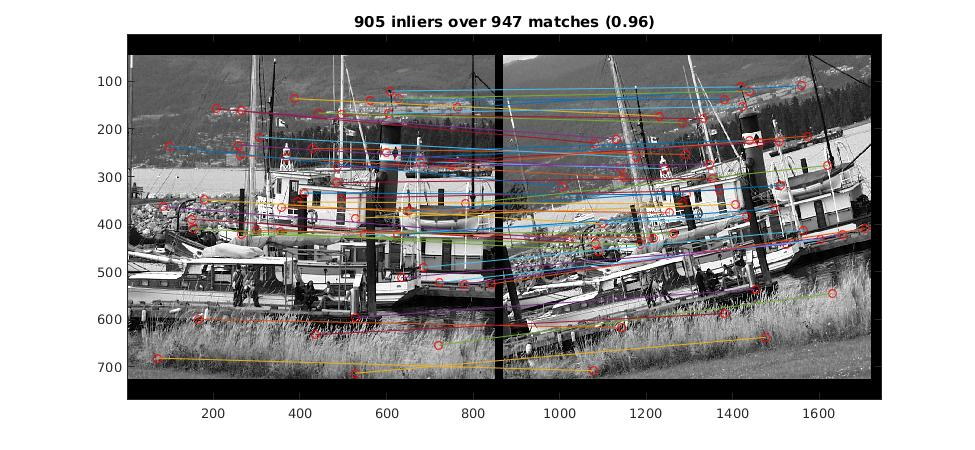
\includegraphics[width=1\textwidth]{imgs/transformed_matches.jpg}
	\caption{Each red dot is a keypoint and the lines connect keypoints that
	match. The keypoints on the right image are the keypoints of the left one, but
	transformed using the affine transformation during RANSAC; the algorithm finds
	a model that fits 905 inliers over 947 total matches.}
	\label{fig:ransac_inliers}
\end{figure}

If the count of inliers is greater than the one of the previous best iteration,
we store the transformation parameters and continue the loop. After $N$ loops
have been executed, the \texttt{ransac} function returns the best set of model
parameters and the count of inliers for each iteration.

In Figure \ref{fig:aligned_im1} we show the first boat image transformed so to
match the alignment of the second boat image. Instead in Figure
\ref{fig:aligned_im2} we show the second boat image aligned to the first one
using the inverted transformation matrix.

\begin{figure}[htpb]
	\centering
	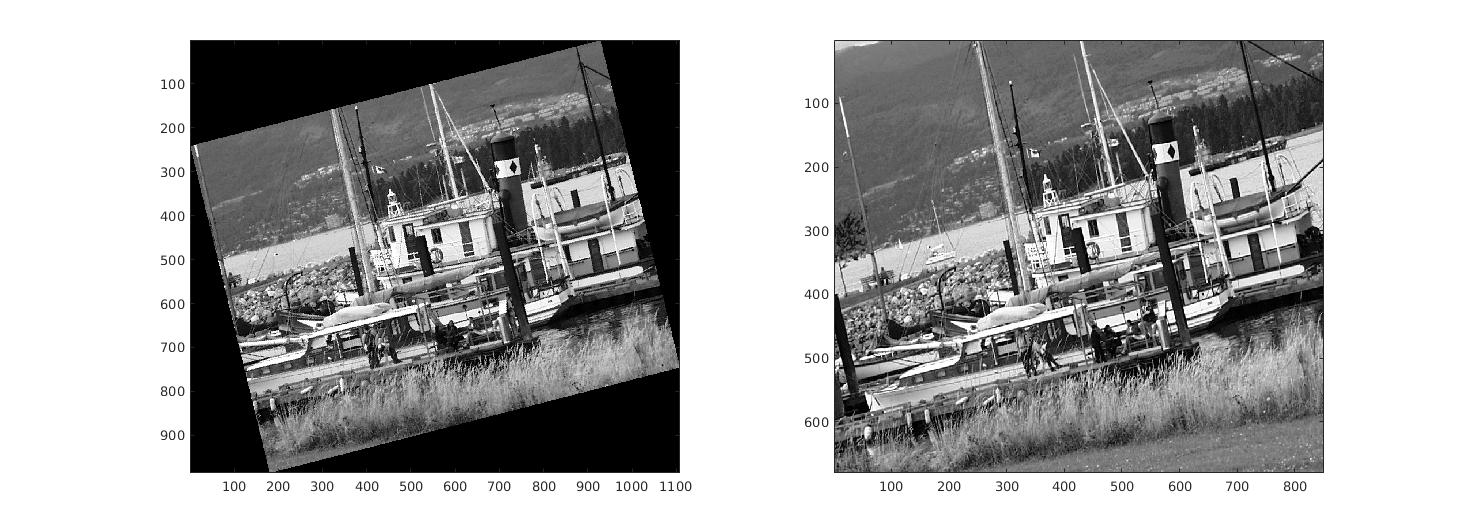
\includegraphics[width=1\textwidth]{imgs/aligned_im1.jpg}
	\caption{First boat image aligned to the second one.}
	\label{fig:aligned_im1}
\end{figure}

\begin{figure}[htpb]
	\centering
	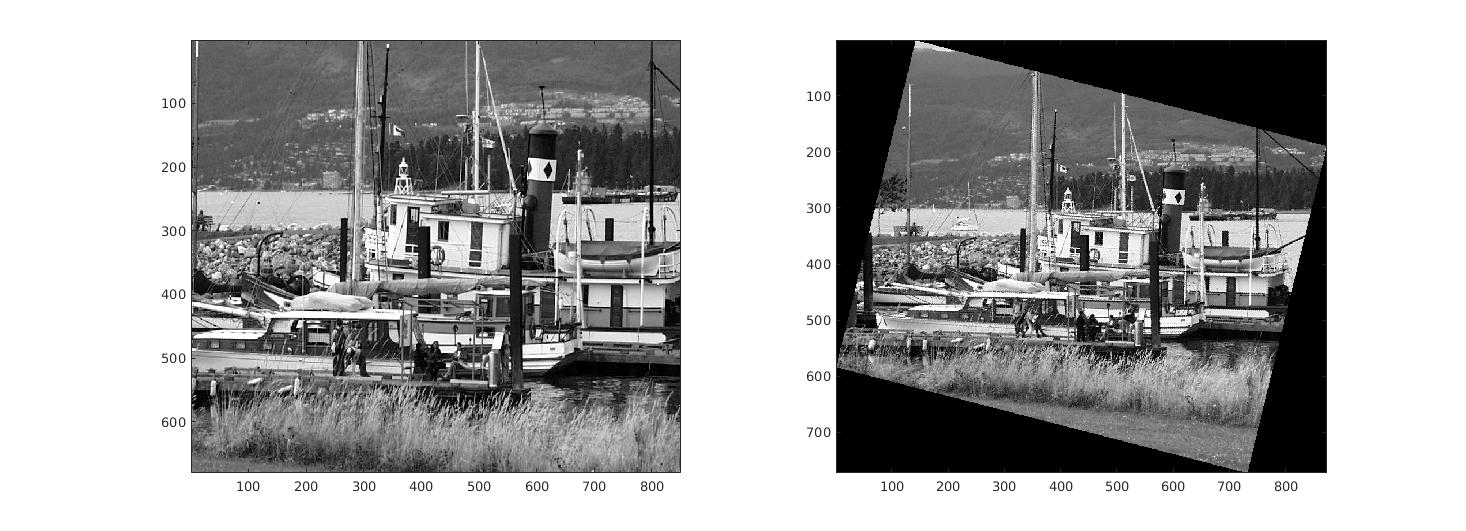
\includegraphics[width=1\textwidth]{imgs/aligned_im2.jpg}
	\caption{Second boat image aligned to the first one.}
	\label{fig:aligned_im2}
\end{figure}

% TODO discuss about N
% N > log(1 - p) / log(1 - (1 - e)^s)
By using the following formula we can compute how sufficiently big $N$ has to be
in order to have a likelihood of success, let's say, of $p = 0.99$.

\begin{equation}
	N > \frac{\ln(1 - p)}{\ln(1 - (1 - e)^P)}
	\label{eq:ransac_n}
\end{equation}

In equation \ref{eq:ransac_n} $p$ is the likelihood of success, $e$ is the
percentage of outliers (so $1 - e$ is the percentage of inliers) and $P$ is the
sample size ($P = 3$ in our case). Suppose we have $e = 0.5$, so that we expect
to encounter 50\% of outliers, we can plug in those values and find a minimum
value for $N$ that guarantees us to find the best set of parameters with a
probability of 99\%, which is $34.5$.

% TODO differences between our image transformation fn and matlab's imtransform

\section{Image Stitching}


\end{document}
